


% This LaTeX was auto-generated from an M-file by MATLAB.
% To make changes, update the M-file and republish this document.






  
    

\section{RFEM Slice Tester} \label{sec:RFEMTests}
Testing results obtained from the RFEMSolver.m program, a module in
the SSA program. Factor of safety results from the program are
compared to results from examples in slope stability papers, to judge the
accuracy of the implemented algorithm. As seen mentioned in the
Morgenstern Price solver testing (section \ref{sec:MPTests}), due to the
imperfect nature of the comparisons, results are judged on a relative
basis. Example numbers refer to the same slope/slip problem as
analyzed in the Morgenstern Price tests. The comparisons from scientific
papers were performed using non RFEM solver algorithms, such as
Morgenstern Price or Spencer's method. Therefore the relative accuracy of
the implemented Morgenstern Price algorithm may appear higher, this does
not also suggest the Morgenstern Price solver is truly more accurate
however. Ideally and as is seen the RFEM solver should converge to a
solution similar to the comparison slip, as two different methods
calculating similar answers suggest accuracy of both methods.

\subsection{Example 1}
Results compared to those from Greco (1996), Malwaki et al (2001),
Cheng et al(2007), and Li et al (2010). A graph of the relative error
between the factor of safety calculated by the program with the factor of
safety given in the papers is used to analyze the results. The results
using the Morgenstern Price algorithm is also plotted. As the comparison
was also performed using the Morgenstern Price algorithm this relative
error is almost 0.


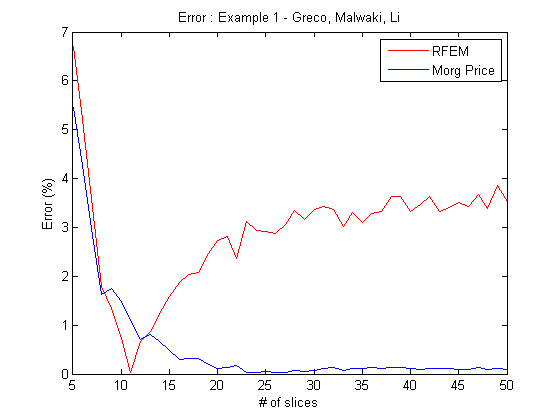
\includegraphics [width=5in]{./VV_SubDocuments/RFEMSliceTester_01.png}



The figure shows convergence to a consistent relative error of less than
5\% after approximately 25 slices for the RFEM solver. This is a positive
result suggesting accuracy of both methods. However as seen in the
following figure the RFEM algorithm requires significantly more
computation time than the Morgenstern Price algorithm (section
\ref{sec:MPTests}). The large difference in calculation time makes the
Morgenstern Price solver much more efficient, especially when performing
repeated analysis in the Genetic Algorithm search.


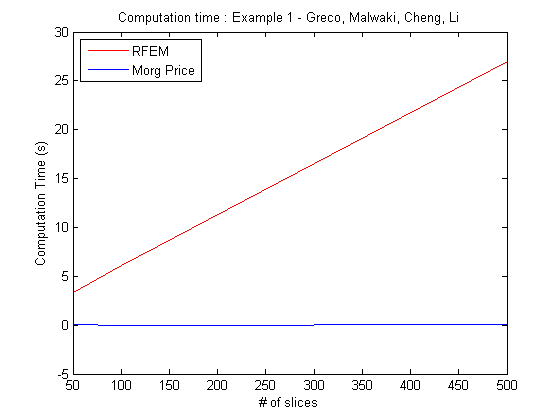
\includegraphics [width=5in]{./VV_SubDocuments/RFEMSliceTester_02.png}



\subsection{Examples 2 and 6}
Results compared to those from Zolfaghari et al (2005), Cheng et al
(2007), Li et al (2010) and Pham and Fredlund (2003). The graphs of these
examples continue to show convergence to relative error of approximately
5\% - 10\% after approximately 25 steps. Again these are all positive
results suggesting accuracy of both solvers.


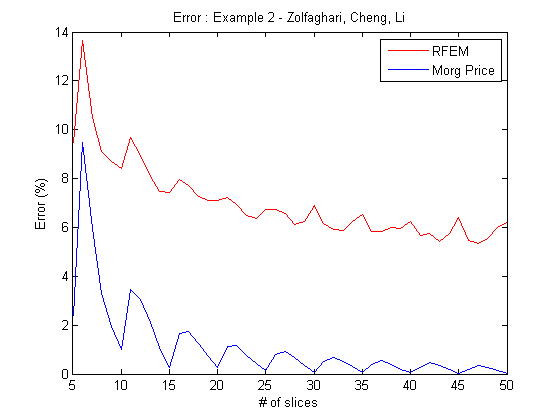
\includegraphics [width=5in]{./VV_SubDocuments/RFEMSliceTester_03.png}




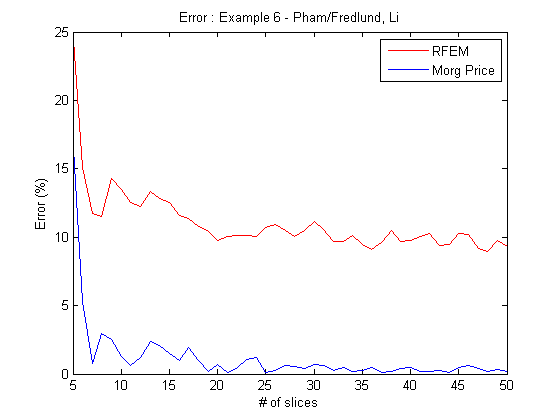
\includegraphics [width=5in]{./VV_SubDocuments/RFEMSliceTester_04.png}


